\chapter{Organisation}
Dette kapitel omhandler opbygningen af organisationen, hvori teknologien implementeres. I kapitlet undersøges tilrettelæggelse og opgavefordeling i de afdelinger af sundhedssektoren, som påvirkes ved indførelse af Fitbit Flex.

\section{Metode}
Det ønskes at undersøge de organisatoriske forudsætninger samt mulige konsekvenser ved implementering af Fitbit Flex til monitorering i den primære sektor. Undersøgelsen tager udgangspunkt i den modificerede Leavitt organisationsmodel på \autoref{fig:leavittmodel}, for at analysere konsekvenserne af en eventuel ændring i organisationen. Leavitts modificerede organisationsmodel benyttes, da denne tager højde for omgivelsernes påvirkning på teknologi, aktører, opgaver, struktur, disses indbyrdes påvirkning og påvirkning på omgivelserne.

\begin{figure}[H]
\centering
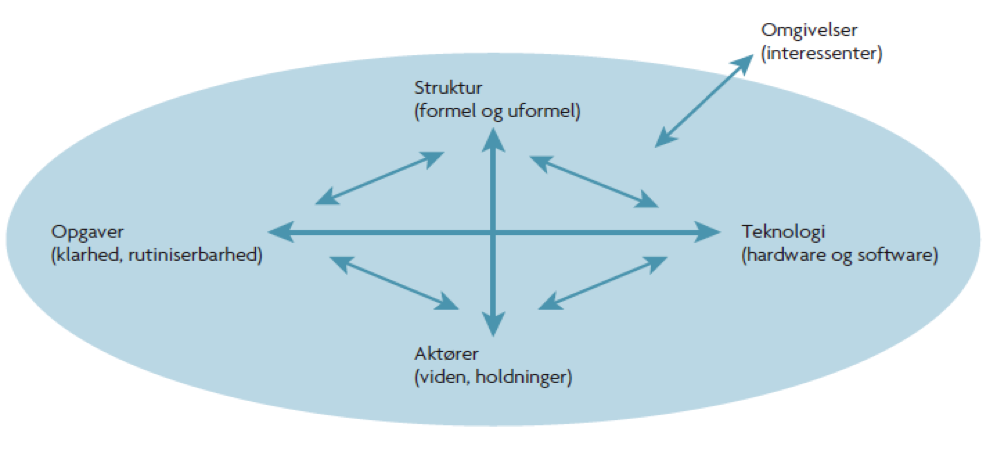
\includegraphics[width=0.9\textwidth]{figures/leavitt}
\caption{Leavitts modificerede organisationsmodel \citep{mtvhaandbog}.}
\label{fig:leavittmodel}
\end{figure}
\noindent
Dette giver anledning til følgende MTV-spørgsmål:

\subsection{MTV-spørgsmål}
\begin{itemize}
\item Hvordan passer Fitbit Flex ind i den primære sundhedssektor? 
\item Hvilke krav vil implementeringen stille til alment praktiserende læger, og hvem skal stå for en eventuel efteruddannelse? 
\item  Hvordan vil patientfordelingen mellem den primære og sekundære sundhedssektor blive påvirket, og hvad vil en ændring i arbejdsfordelingen medføre?
\item Hvilken effekt har anvendelsen af Fitbit Flex til dokumentation af aktivitietsniveau på patientens sygdom?
\end{itemize}